% Built from the official Tech Science Press LaTeX template.
\documentclass[cmc,article,submit,moreauthors,pdftex]{Definitions/tsp}
\input{Definitions/package}
\input{Definitions/unicode}
\usepackage{longtable}
\usepackage{url}
\providecommand{\tightlist}{\setlength{\itemsep}{0pt}\setlength{\parskip}{0pt}}
\graphicspath{{./Definitions/}{./figures/}}

\continuouspages{}
\firstpage{1}
\makeatletter\setcounter{page}{\@firstpage}\makeatother
\pubvolume{0}\issuenum{0}\elocationid{0}\articlenumber{0}
\pubyear{2026}\doiyear{2026}\copyrightyear{2026}
\datereceived{Day Month Year}\dateaccepted{Day Month Year}
\dateonlinefirst{}\datepublished{Day Month Year}
\Title{A Decision-Consequence Auditing Framework for Reliable Surrogate-Assisted Optimization in Expensive Engineering Design}
\Author{Shu-Chuan Chu\textsuperscript{1,*}, Ya-Yu Zhang\textsuperscript{1}, Zhenyu Meng\textsuperscript{2} and Zhao Jia\textsuperscript{3}}
\AuthorNames{Shu-Chuan Chu, Ya-Yu Zhang, Zhenyu Meng and Zhao Jia}
\address{\textsuperscript{1}School of Computer Science, Nanjing University of Information Science and Technology, Nanjing 210044, Jiangsu, China

\textsuperscript{2}Affiliation to be confirmed for Zhenyu Meng

\textsuperscript{3}Affiliation to be confirmed for Zhao Jia

Ya-Yu Zhang: 202412492223@nuist.edu.cn

Zhenyu Meng: mzy1314@gmail.com

ORCID: Shu-Chuan Chu, \href{https://orcid.org/0000-0003-2117-0618}{0000-0003-2117-0618}; Ya-Yu Zhang, \href{https://orcid.org/0009-0001-2272-4654}{0009-0001-2272-4654}; Zhenyu Meng, \href{https://orcid.org/0000-0002-1466-8082}{0000-0002-1466-8082}; Zhao Jia, \href{https://orcid.org/0000-0002-3652-1903}{0000-0002-3652-1903}}
\corres{Corresponding Author: Shu-Chuan Chu. Email: 100130@nuist.edu.cn}
\abstract{Reliable surrogate-assisted optimization requires more than an accurate predictor: surrogate information must alter model-management decisions in ways that improve outcomes under a limited expensive-evaluation budget. A decision-consequence auditing framework is developed to evaluate this pathway systematically. The framework separates three questions: whether a monitoring signal is calibrated on the data it encounters, whether it changes candidate selection and improves immediate utility at a common optimization state, and whether the resulting closed loop improves final optimization. It combines decision-pathway analysis, prediction-before-label records, common-state comparisons, and independent closed-loop validation with a promotion-or-stop gate. A temporal residual monitor is used as a representative case study. For its candidate-independent additive correction, ranking invariance is established under identical candidate sets, deterministic tie-breaking, exact arithmetic, and synchronized stochastic operators. The audit then shows that its effective pathway is an exploration controller rather than a distinct exploitation ranking. Across all 24 noiseless BBOB functions in dimensions 10, 20, and 40, the monitored controller does not pass the prespecified optimization-benefit gate despite a failure fraction near its nominal level. Application validation on a 200-evaluation finite-element Messerschmitt-Bolkow-Blohm beam design reaches the same mechanism conclusion. Under a shared 58-point initialization, GP-PI, author-code DRSO, and TuRBO-1 reduce median compliance by 51.7\%, 74.7\%, and 75.1\%, whereas GP-EI and fixed-multiplier GP-UCB show no median improvement. The resulting contribution is a reusable reliability-assessment procedure that distinguishes predictive calibration from decision influence, decision utility, and closed-loop value before large simulation or engineering budgets are committed.}
\keyword{expensive black-box optimization; surrogate-assisted evolutionary optimization; model management; prequential residuals; finite-element design}
\begin{document}
\hypertarget{introduction}{%
\section{Introduction}\label{introduction}}

Many engineering optimization problems depend on simulations, model training, or experiments whose evaluations dominate the available computational or physical budget. Surrogate-assisted evolutionary algorithms and Bayesian optimization reduce this burden by fitting an inexpensive predictive model and deciding which candidate should receive the next exact evaluation \cite{ref-1,ref-2,ref-3,ref-4,ref-5}. Model management is therefore the operational core of surrogate assistance: surrogate prediction is converted into an acquisition or management decision, that decision allocates a paid evaluation, and the resulting label changes the subsequent optimization state. A reliable predictor is useful only when this chain improves the use of the available budget.

This distinction matters directly in finite-element structural optimization, topology-oriented design, materials and manufacturing parameter selection, robotics, and neural architecture search. In these settings, an apparently reasonable uncertainty or error signal can redirect many costly simulations or experiments. Recent CMC studies illustrate this engineering breadth through hierarchical surrogate evaluation for neural architecture search \cite{ref-27}, deep-surrogate multi-objective robotic linkage design \cite{ref-28}, and physics-informed Gaussian-process Bayesian optimization supported by finite-element welding analysis \cite{ref-29}. Surrogate assistance has also been integrated with bimodal particle-swarm search for computationally expensive multi-UAV path planning \cite{ref-33}, demonstrating how model-management choices affect a safety- and resource-constrained engineering application. The beam application studied here places reliability auditing inside the same class of expensive engineering decisions rather than treating it as an abstract diagnostic exercise.

Recent methods use Gaussian-process uncertainty, ensembles, local models, temporal information, or adaptive infill rules to balance exploitation and exploration \cite{ref-6,ref-7,ref-8,ref-9,ref-10,ref-11}. Online and conformal calibration research asks whether predictive distributions or bounds retain their intended reliability under sequential selection \cite{ref-12,ref-13,ref-14,ref-15}. Calibration alone, however, does not establish that a signal changes candidate ordering, selects a better candidate at the same state, or improves a closed-loop trajectory after the surrogate and candidate distribution adapt. These properties form a decision pathway and must be evaluated separately.

A decision-consequence auditing framework is developed for that purpose. The representative temporal post-selection error monitor records predictions before labels, estimates an empirical residual bound, and converts failures, bound width, and stagnation into spatial exploration. The framework is not tied to that monitor: it accepts any surrogate, candidate generator, monitoring signal, and acquisition or model-management rule whose pathway to paid evaluations can be inspected. The monitored controller supplies a demanding case because its calibration diagnostic appears plausible while its decision pathway contains an algebraically redundant exploitation term.

The major contributions are as follows.

\begin{enumerate}
\def\labelenumi{\arabic{enumi}.}
\tightlist
\item
  A decision-consequence auditing framework is developed to determine whether surrogate monitoring signals influence model-management decisions and whether those decisions improve expensive optimization.
\item
  A ranking-invariance criterion is established for candidate-independent additive corrections. Under explicit candidate-set, tie-breaking, arithmetic, random-stream, stochastic-operator, and state-update conditions, such a correction cannot create a distinct exploitation ranking.
\item
  A three-level validation protocol separates common-history calibration, common-state decision influence and utility, and independent closed-loop optimization. Prediction-before-label journals preserve the information boundary, while a promotion-or-stop gate prevents diagnostic performance from being reported as optimization value.
\item
  The framework is evaluated across BBOB, LassoBench, a 300-dimensional extension, and a finite-element structural design application. Matched-initialization GP-EI, GP-PI, GP-UCB, author-code DRSO, and TuRBO-1 comparisons distinguish initialization effects from acquisition behavior and provide successful and unsuccessful surrogate-management controls.
\end{enumerate}

Algorithm 1 is the algorithmic contribution of this study: it is an executable predeployment procedure for accepting, revising, or stopping a surrogate-management mechanism. The temporal residual monitor is an audited case study rather than a newly proposed optimizer.

The claims are deliberately bounded. The empirical residual quantile is not presented as a conformal coverage theorem, false-discovery guarantee, regret bound, or universally effective high-dimensional method. The case-study findings concern a deterministic, single-objective setting, the stated surrogate and candidate process, and the tested budgets. The framework itself supplies a structured test procedure; it does not imply that candidate-dependent uncertainty, expected improvement, confidence bounds, restarts, stopping rules, or uncertainty-aware optimization in general are ineffective.

\hypertarget{related-work}{%
\section{Related Work}\label{related-work}}

\hypertarget{surrogate-assisted-optimization-and-engineering-applications}{%
\subsection{Surrogate-assisted optimization and engineering applications}\label{surrogate-assisted-optimization-and-engineering-applications}}

Surrogate-assisted evolutionary computation has developed a broad range of models and management policies for expensive optimization \cite{ref-1,ref-2}. Early frameworks combined evolutionary search with approximate fitness functions or Gaussian-process surrogates \cite{ref-3,ref-16}. Later work introduced selective ensembles, local/global models, classification-assisted search, and adaptive infill rules \cite{ref-4,ref-5,ref-17,ref-18,ref-19}. Differential evolution remains a common search engine in this area; the taxonomy and empirical evidence synthesized by Pan et al.~\cite{ref-31} show that exponential-crossover behavior depends strongly on operator design and parameter control. A recent survey identifies model construction and model management as separate determinants of performance \cite{ref-2}. Controlled experiments with adjustable surrogate accuracy likewise show that prediction accuracy affects preselection, individual-based, and generation-based management differently \cite{ref-20}.

CMC applications show how these ideas enter expensive computational workflows. Hierarchical surrogate evaluation reduces neural-architecture search cost \cite{ref-27}, deep surrogate models support multi-objective robotic linkage design \cite{ref-28}, and physics-informed Gaussian-process regression with adaptive Bayesian optimization combines finite-element knowledge with welding-parameter selection \cite{ref-29}. These studies motivate reliability checks at the decision layer because prediction accuracy and evaluation savings are valuable only when surrogate outputs lead to useful paid evaluations.

Uncertainty-aware SAEAs typically make uncertainty candidate dependent. BGP-SAEA combines a boosting framework with Gaussian-process uncertainty \cite{ref-6}, while recent large-scale methods use lower-confidence-bound Gaussian-process models and diversity search \cite{ref-7}. For expensive multi-objective optimization, MLPSGP-SAEA combines multilayer-perceptron variable grouping, sparse Gaussian processes, and an adaptive sparse-and-diverse infill criterion \cite{ref-32}. Other work adapts differential-evolution selection to errors in both decision and objective spaces \cite{ref-8}, tightens the search space for high-dimensional expensive problems \cite{ref-9}, or draws on multiple spatial, temporal, and performance information sources \cite{ref-10}. These mechanisms can change candidate ranking, local search regions, or population updates.

Competitive SAEAs also use evolutionary populations and learned relations rather than a scalar acquisition alone. DRSO retains unevaluated promising solutions in a relation-model-assisted evolutionary loop to preserve useful population information under expensive-evaluation budgets \cite{ref-30}. Its public author implementation makes it suitable for a source-frozen engineering comparison, while its distinct population mechanism broadens the evidence beyond Gaussian-process acquisitions.

\hypertarget{reliability-aware-surrogate-model-management}{%
\subsection{Reliability-aware surrogate model management}\label{reliability-aware-surrogate-model-management}}

Bayesian optimization has incorporated online calibration. Deshpande et al.~\cite{ref-12} calibrate predictive distributions and update them online. Localized online conformal Bayesian optimization constructs spatially varying thresholds and a calibrated posterior \cite{ref-13}. Selection-conditional methods such as JOMI use reference sets under explicit invariance and exchangeability conditions \cite{ref-14}. Temporal conformal prediction has also been considered in surrogate-assisted evolutionary optimization \cite{ref-15}. The cross-model residual journal examined here does not establish the assumptions required by those methods and is treated as an empirical monitor without transferred guarantees.

\begin{table}[H]
\tablesize{\scriptsize}
\caption{Scope of representative reliability and model-management approaches.}
\label{tab:main-1}
\centering
\begin{adjustbox}{max width=\textwidth}
\begin{tabular}{lrrr}
\toprule
\textbf{Approach} & \textbf{Primary quantity assessed} & \textbf{Direct decision question} & \textbf{Closed-loop consequence required} \\
\midrule
Gaussian-process uncertainty & Predictive confidence & Does uncertainty modify an acquisition value? & Usually evaluated by optimizer performance \\
Conformal prediction & Marginal or localized coverage & Does a calibrated set or bound satisfy its stated guarantee? & Not implied by coverage alone \\
Adaptive infill & Evaluation selection & Which candidate receives the next expensive label? & Evaluated through search performance \\
Candidate-dependent SAEA management & Ranking, region, or population update & Does surrogate information change the search action? & Method-specific \\
Relation-model DRSO & Pairwise fitness/category relations and unevaluated population & Does evolutionary surrogate management preserve promising search information? & Evaluated by paid-budget endpoint \\
Decision-consequence audit & Calibration, decision influence, utility, and final outcome & Does the signal change a paid decision and make it more useful? & Required as the final audit level \\
\bottomrule
\end{tabular}
\end{adjustbox}
\end{table}

Several studies compare Bayesian, evolutionary, and hybrid surrogate strategies under constrained budgets \cite{ref-21}, and others show that unevaluated but surrogate-predicted candidates can influence evolutionary diversity \cite{ref-22}. The present framework is complementary to these optimizers. It evaluates the sequence from a surrogate-derived signal to model-management action, common-state utility, and independent closed-loop consequence. This taxonomy identifies the gap between a reliable predictive quantity and a reliable optimization decision.

\hypertarget{decision-consequence-auditing-framework-for-surrogate-assisted-model-management}{%
\section{Decision-Consequence Auditing Framework for Surrogate-Assisted Model Management}\label{decision-consequence-auditing-framework-for-surrogate-assisted-model-management}}

\hypertarget{optimization-system-and-information-boundary}{%
\subsection{Optimization system and information boundary}\label{optimization-system-and-information-boundary}}

A deterministic objective f(x) is minimized over a bounded continuous domain under budget B. At evaluation t, the labeled history contains only observations acquired before t. A surrogate fitted to that history supplies predictions for a candidate set, while a monitoring signal and model-management rule determine which candidate, region, evaluation gate, restart, or stopping action is used. The audit treats the full chain from surrogate output to paid evaluation as its object of analysis.

Before the objective is called, a prediction-before-label journal stores the candidate set or its reproducible identifier, selected point, surrogate outputs, monitoring signal, incumbent, decision mode, support indicators, and random-state identifiers. The record is flushed before the label is obtained. Labels acquired solely for frozen-state diagnostics remain separate and never return to the optimizer. This boundary prevents outcome information from leaking into the decision being audited.

The role of the framework in a surrogate-assisted optimization loop is shown in Figure 1.

\begin{figure}[H]
\centering
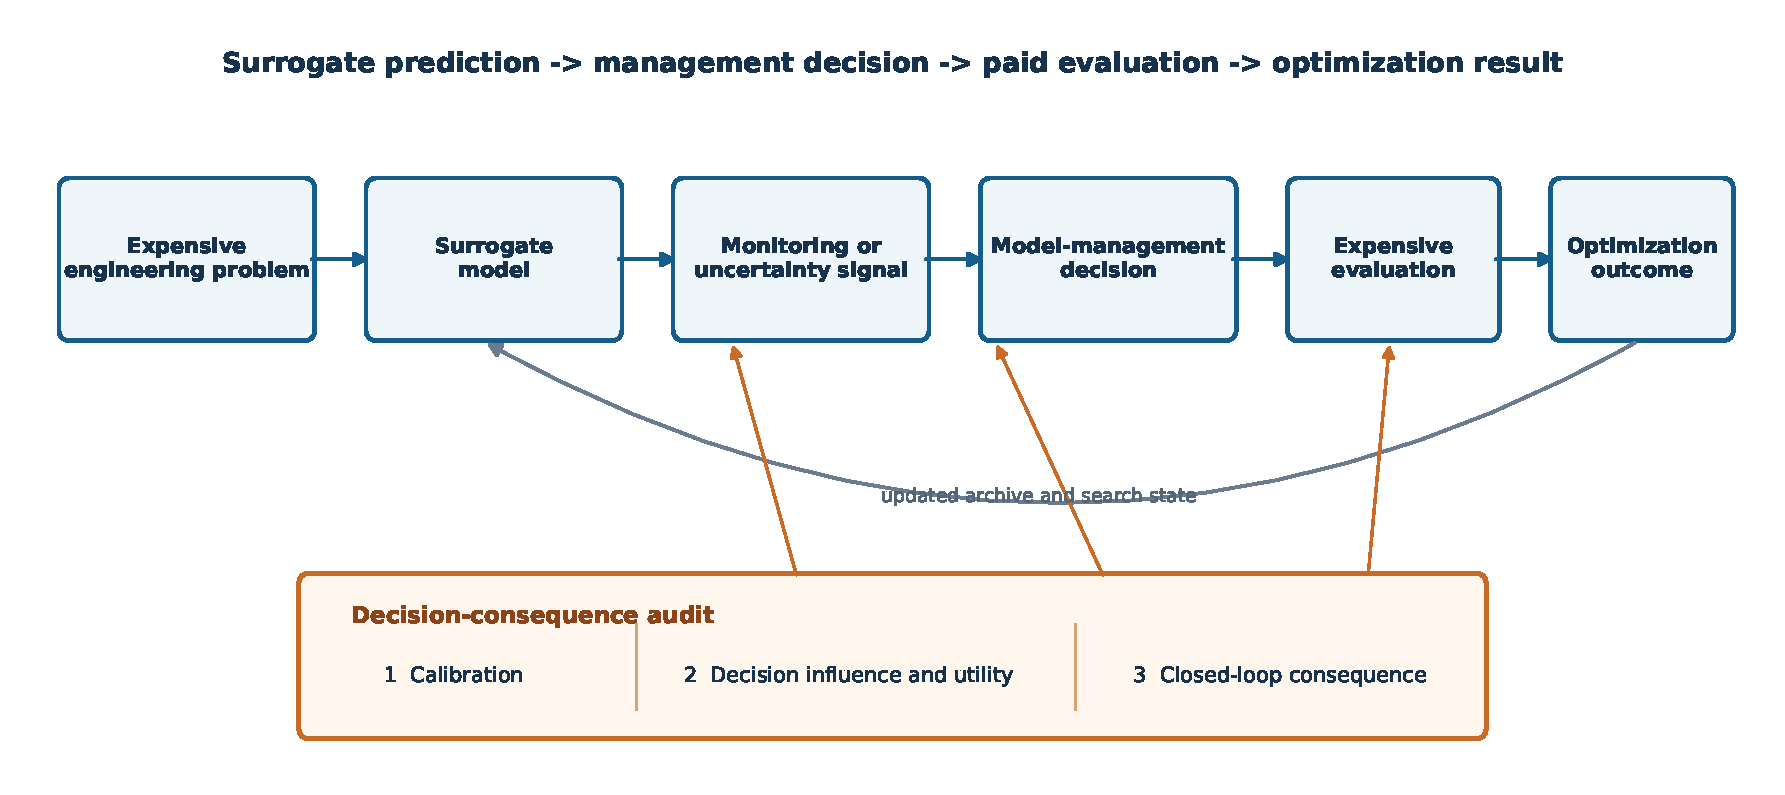
\includegraphics[width=0.92\textwidth]{figures/main_figure_1.pdf}
\caption{Decision-consequence auditing framework for surrogate-assisted optimization.}
\label{fig:main-1}
\end{figure}

Figure 1 locates the three audit levels along the operational chain from an expensive engineering problem to surrogate prediction, model-management choice, paid evaluation, and closed-loop outcome. Calibration assesses the signal encountered by the optimizer; decision analysis tests whether the signal changes a choice and improves common-state utility; closed-loop validation measures the final consequence after histories diverge.

\hypertarget{decision-pathways-and-ranking-invariance}{%
\subsection{Decision pathways and ranking invariance}\label{decision-pathways-and-ranking-invariance}}

A monitoring mechanism can affect optimization through candidate-specific ranking, an evaluation gate, a restart or stopping rule, a change of search region or population, or a stochastic exploration controller. The first audit step identifies at least one such path before additional expensive experiments are authorized.

\textbf{Lemma 1 (ranking invariance under a candidate-independent additive correction).} At evaluation t, suppose two rules receive an identical indexed candidate set, use deterministic and identical tie-breaking, and are evaluated in exact arithmetic. If every supported candidate shares the same additive correction c\_t, then minimizing H\_t(x)=mu\_t(x)+c\_t returns the same minimizer index as minimizing mu\_t(x).

\textbf{Proof.} For any indexed candidates x\_i and x\_j, H\_t(x\_i)-H\_t(x\_j)=mu\_t(x\_i)-mu\_t(x\_j). Every strict comparison and exact tie is therefore preserved under the stated tie-breaking rule. The same indexed minimizer follows. \(\square\)

\textbf{Corollary 1.} If two configurations also share initialization, candidate generation, exploration decisions, all random streams and stochastic operators, numerical precision, and optimizer-state updates, and differ only by replacing the common-correction minimizer with the mean minimizer, their trajectories are identical by induction over evaluations. Finite-precision agreement is an implementation property and is checked separately in the experiment audit.

This result identifies a structural limitation of candidate-independent corrections; it does not invalidate uncertainty-aware surrogate management in general. Candidate-dependent posterior uncertainty, expected improvement, lower-confidence bounds, support-dependent rules, evaluation gates, restarts, and stopping policies may create decision paths that Lemma 1 does not remove.

\hypertarget{three-audit-levels-and-promotion-gate}{%
\subsection{Three audit levels and promotion gate}\label{three-audit-levels-and-promotion-gate}}

Common-history calibration fits the same frozen model and candidate pool, then evaluates monitoring losses and failures without updating the search. Common-state decision analysis compares the action with and without the mechanism at the same state; when actions differ, separate diagnostic labels measure true one-step utility. Independent closed-loop experiments then allow each policy to update its own history and evaluate final optimization behavior. A mechanism advances only when evidence from the cheaper level justifies the next.

\textbf{Algorithm 1. Decision-consequence audit for a surrogate-assisted model-management mechanism.}

\textbf{Step 1 --- Specify.} Freeze the surrogate, candidate generator, monitoring signal, management or acquisition rule, expensive objective, budget, and deterministic replay information. Output: protocol and information boundary.

\textbf{Step 2 --- Trace.} Follow the signal through ranking, evaluation, region, population, restart, stopping, or stochastic-exploration decisions. Gate: at least one candidate-dependent or otherwise actionable path.

\textbf{Step 3 --- Record and calibrate.} Persist every decision before its label and audit common-history calibration on separated diagnostic data. Gate: supported calibration evidence with no label leakage.

\textbf{Step 4 --- Test common-state utility.} Freeze optimization states, compare baseline and monitored actions, and label alternatives only in the diagnostic archive. Gate: demonstrated decision change and common-state utility.

\textbf{Step 5 --- Validate the closed loop.} When the pathway and utility gates pass, run independent optimization on held-out instances or applications under the same paid budget. Output: final objective consequence.

\textbf{Step 6 --- Decide.} Promote, revise, or stop the mechanism and report the first failed gate with its evidence boundary. Output: stage-wise audit record.

The framework can return a positive result. Classical GP expected improvement is a candidate-dependent positive control: both its predicted improvement and uncertainty vary across candidates, so its acquisition can change ranking and passes the structural decision-influence check. Passing that first check does not guarantee superior endpoints; it authorizes empirical utility and closed-loop evaluation.

\hypertarget{experimental-design}{%
\section{Experimental Design}\label{experimental-design}}

\hypertarget{representative-monitored-optimizer-and-search-framework}{%
\subsection{Representative monitored optimizer and search framework}\label{representative-monitored-optimizer-and-search-framework}}

A temporal residual monitor is used as the representative audited mechanism. For a selected point x\_t, the standardized signed residual is r\_t={[}y\_t-mu\_t(x\_t){]}/s\_t, where s\_t is the standard deviation of the current training labels and is replaced by one if it is zero. Historical residuals retain their prediction-time models and scales. For candidate x, the monitor forms H\_t(x)=mu\_t(x)+s\_t q\_t(x), where q\_t(x) is the nonnegative weighted 0.9 quantile of at most the latest 100 residuals. Temporal weights have a half-life of 25 evaluations; spatial variants use a Gaussian kernel and an effective-sample-size support guard of 20.

The temporal prototype PEM-T converts recent failures, normalized bound width, and evaluations without incumbent improvement into an exploration probability between 0.1 and 0.8. Exploration selects the candidate with the largest minimum distance to the archive. Otherwise, the smallest supported upper value is used when an improvement declaration is available and the monitor is not alarmed; the smallest predicted mean is used in the remaining cases. Fixed01 retains the same model and candidate process with exploration probability 0.1. Under the temporal bound, q\_t and s\_t are common to supported candidates, so Lemma 1 predicts that the upper-value and mean exploitation rankings coincide.

The internal optimizer uses a randomized Latin hypercube with 2D+20 initialization points. The first D+10 points train the initial model; the remaining D+10 are predicted before labeling and create startup residuals. Inputs are scaled to the unit cube. A regularized Gaussian radial-basis-function surrogate uses distance divided by the square root of D, length scale 0.25, ridge $10^{-6}$, and standardized labels. At most 256 observations are retained through an elite-plus-farthest-point rule.

Each iteration proposes 256 candidates: 128 reflected differential-evolution proposals and 128 scrambled Sobol points. Duplicates and candidates within $10^{-10}$ of evaluated points are replaced. Purpose-specific random streams depend on seed and evaluation index rather than the total budget.

\hypertarget{development-and-independent-validation}{%
\subsection{Development and independent validation}\label{development-and-independent-validation}}

Development uses eight prespecified BBOB functions, dimensions 10 and 20, instances 1-3, and three repeats. Thirteen internal configurations separate exploration, residual weighting, and feedback components. The budget is 10D. The required gate compares PEM-T with a fixed exploration control selected only within the development protocol. Failure of the gate prevents any optimization-superiority claim.

After the gate fails, the unchanged mechanism is frozen on all 24 noiseless BBOB functions, dimensions 10, 20, and 40, instances 11-13, and three repeats. Six internal configurations produce 3,888 runs and 907,200 paid evaluations. Three history policies produce 7,776 frozen states and 1,990,656 diagnostic labels. Development and validation estimates are never pooled.

The endpoint is the base-10 logarithm of final error relative to common initialization error, with numerical flooring at $10^{-12}$. Repeats are summarized within function-instance cells, instances are averaged, and functions receive equal weight. Nine prespecified validation contrasts form one Holm family. Paired hierarchical bootstrap intervals resample functions, instances, and common repeat indices. These intervals summarize suite heterogeneity and are not presented as a population theorem for all black-box tasks.

\hypertarget{external-and-application-evidence}{%
\subsection{External and application evidence}\label{external-and-application-evidence}}

Sobol, CMA-ES, classical GP expected improvement, and author-code TuRBO-1 provide budget-matched descriptive references \cite{ref-25}. They retain their own initialization and search mechanisms, so these comparisons are not same-history causal effects. In the finite-element application, GP expected improvement (GP-EI), probability of improvement (GP-PI), and the lower-confidence-bound form of GP-UCB are additionally run from the same initial observations as the internal methods. All three acquisitions use the same Matérn-5/2 Gaussian process, candidate pool, and local-search budget; GP-PI uses a margin equal to 0.01 times the observed response standard deviation, and GP-UCB uses a fixed confidence multiplier of 2.0. DRSO uses the authors' public relation-model-assisted evolutionary implementation at commit 03c19d4 \cite{ref-30}. The population size is set to 58 solely to accept the common initial archive; its relation models, unevaluated-population update, reproduction, training cap, and remaining defaults are unchanged. Three LassoBench tasks provide application transfer under fixed data and splits \cite{ref-24}. The BBOB implementation and reporting follow the COCO comparison framework \cite{ref-26}. Complete tables, the 300-dimensional extension, resource measurements, sensitivity studies, interruption accounting, and file-level audits appear in the Supplementary Materials.

\hypertarget{mechanism-results}{%
\section{Mechanism Results}\label{mechanism-results}}

\hypertarget{development-gate-and-implementation-invariants}{%
\subsection{Development gate and implementation invariants}\label{development-gate-and-implementation-invariants}}

All 1,872 development optimization runs and 432 common-history runs complete without exceptions. PEM-T and the configuration that removes its upper-value mode have identical trajectories in all 144 matched pairs. Temporal monitoring with fixed 0.3 management likewise matches fixed 0.3 mixing in all 144 pairs. These are implementation confirmations of Lemma 1 and Corollary 1, rather than independent effective components.

The development-selected control is fixed01. PEM-T is worse on all eight development functions in both dimensions. Its function-weighted log-relative endpoint difference is +0.2831 in D=10 and +0.1810 in D=20, where positive values favor fixed01. The required optimization-benefit gate is therefore unmet before the independent validation begins.

\hypertarget{independent-endpoint-and-immediate-decision-effects}{%
\subsection{Independent endpoint and immediate decision effects}\label{independent-endpoint-and-immediate-decision-effects}}

Table 2 reports the nine prespecified validation comparisons. PEM-T increases final relative error in all three dimensions. The base-10 differences correspond to geometric error ratios of 1.468, 1.258, and 1.159 for dimensions 10, 20, and 40. The effect decreases with dimension but remains in the unfavorable direction for 60 of 72 function-level comparisons. Common-state feedback decisions also have lower true immediate improvement than mean-greedy decisions in every dimension.

\begin{table}[H]
\tablesize{\scriptsize}
\caption{Prespecified independent validation contrasts. Endpoint values above zero favor fixed01; immediate values below zero favor mean-greedy selection.}
\label{tab:main-2}
\centering
\begin{adjustbox}{max width=\textwidth}
\begin{tabular}{lrrrrr}
\toprule
\textbf{Dimension} & \textbf{Contrast} & \textbf{Estimate} & \textbf{95\% bootstrap interval} & \textbf{Direction count} & \textbf{Holm p} \\
\midrule
10 & PEM-T minus fixed01 endpoint & 0.1668 & [0.0749, 0.2391] & 22 positive, 2 negative & 5.36e-6 \\
20 & PEM-T minus fixed01 endpoint & 0.0998 & [0.0467, 0.1905] & 19 positive, 5 negative & 0.00170 \\
40 & PEM-T minus fixed01 endpoint & 0.0639 & [0.0130, 0.1123] & 19 positive, 5 negative & 0.00170 \\
10 & Feedback minus mean immediate improvement & -0.0170 & [-0.0431, -0.0067] & 1 positive, 18 negative & 0.00078 \\
20 & Feedback minus mean immediate improvement & -0.0158 & [-0.0352, -0.0079] & 0 positive, 21 negative & 0.00048 \\
40 & Feedback minus mean immediate improvement & -0.0344 & [-0.0630, -0.0100] & 1 positive, 20 negative & 0.00048 \\
\bottomrule
\end{tabular}
\end{adjustbox}
\end{table}

The function-level distribution underlying the aggregate endpoint contrasts is shown in Figure 2.

\begin{figure}[H]
\centering
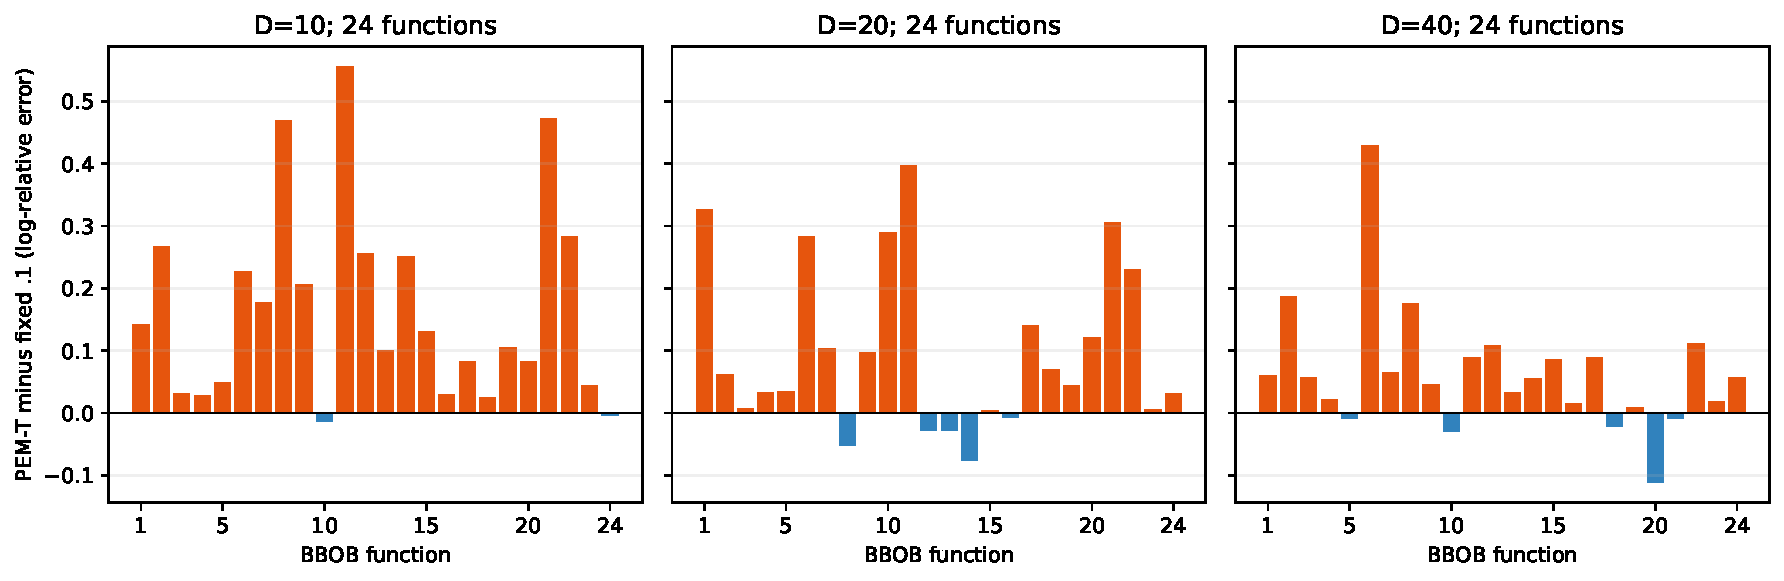
\includegraphics[width=0.92\textwidth]{figures/main_figure_2.pdf}
\caption{Function-level endpoint effects in the independent BBOB validation. Positive values indicate larger PEM-T errors.}
\label{fig:main-2}
\end{figure}

Figure 2 displays all 24 function-level effects separately for each dimension rather than only the suite average. Most bars lie above the zero line: 22 of 24 in dimension 10 and 19 of 24 in both dimensions 20 and 40. The few negative bars show that the result is not pointwise uniform, while the shrinking bar heights across panels agree with the smaller aggregate effect at higher dimension. The conclusion is therefore based on a broad directional pattern with disclosed exceptions, not on one dominant benchmark function.

\hypertarget{calibration-does-not-identify-optimization-utility}{%
\subsection{Calibration does not identify optimization utility}\label{calibration-does-not-identify-optimization-utility}}

PEM-T explores 39.7\%, 36.4\%, and 34.4\% of post-initialization evaluations in dimensions 10, 20, and 40, compared with approximately 10\% for fixed01. Its observed selected-point upper-bound failure fractions are 0.1008, 0.0942, and 0.0964, close to the nominal monitoring level. Nevertheless, its endpoints and common-state decisions are worse. A near-target aggregate failure fraction therefore does not imply efficient budget allocation.

Improvement declarations provide a second example. PEM-T makes 31, 34, and 155 declarations across the three dimensions; 20, 27, and 30 are false. The corresponding pooled false-declaration fractions are 0.645, 0.794, and 0.194. A one-sided failure rate near 0.1 cannot control the conditional error among the small subset declared to improve the incumbent.

History also changes the object being monitored. Under fixed 0.3 mixing, selected-point failures exceed pool failures, whereas under greedy histories the relationship reverses. The prespecified interaction is positive in all three dimensions and passes Holm adjustment. Selection-induced differences should therefore be attributed to the coupled history and policy, not treated as a universal direction of undercoverage.

The reversal of selected-point and pool failure differences across frozen history policies is shown in Figure 3.

\begin{figure}[H]
\centering
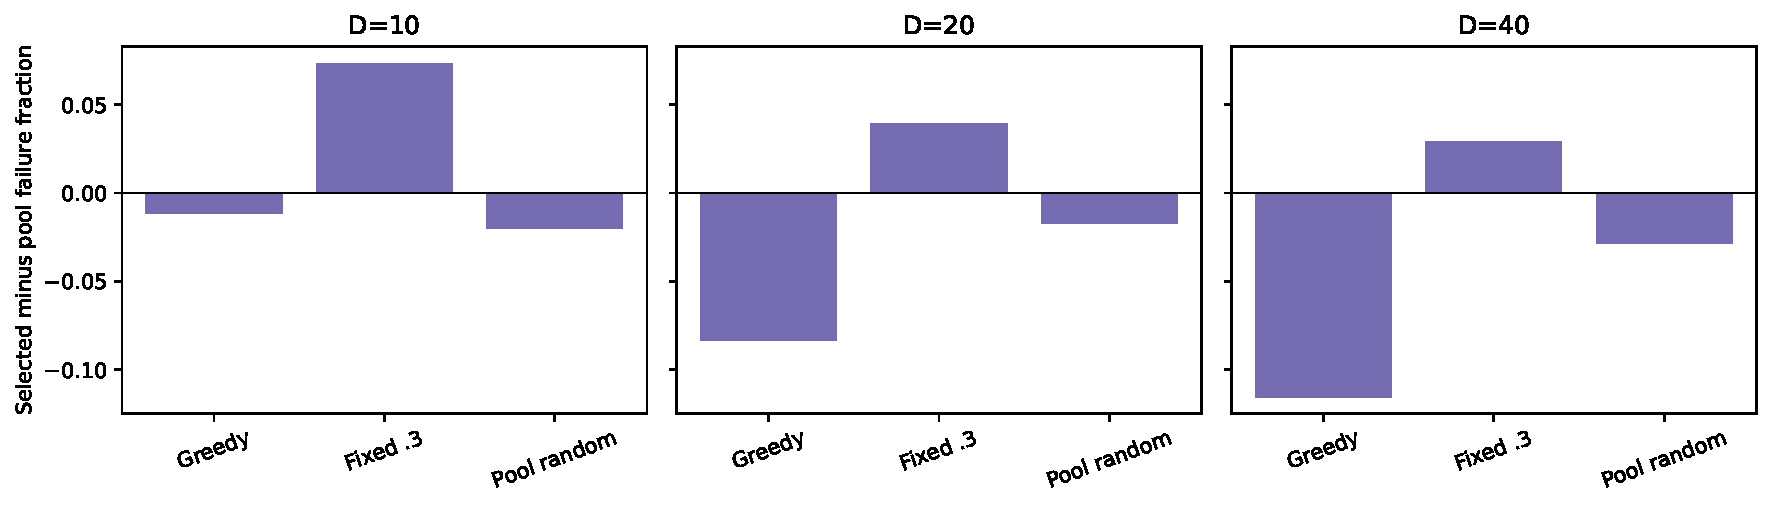
\includegraphics[width=0.92\textwidth]{figures/main_figure_3.pdf}
\caption{Selected-point minus pool failure differences under frozen history policies.}
\label{fig:main-3}
\end{figure}

Figure 3 makes the history dependence visible. Fixed 0.3 histories place the selected-point failure fraction below the pool value in all three dimensions, whereas greedy histories place it above the pool value. Random-pool histories remain closer to zero and are negative in each panel. Because the sign changes with the policy that generated the frozen state, a single universal ``selection penalty'\,' would misrepresent the monitored process.

Spatial-temporal weighting lowers selected-point quantile loss in the prespecified diagnostic comparisons, yet its closed-loop endpoint remains worse than fixed01 in each dimension. This is the central empirical separation: a better residual estimate can still direct evaluations toward candidates with low optimization value.

To isolate the evidential role of each audit stage, a stage-omission ablation is constructed from the frozen records. Unlike an optimizer-component ablation, omitting an audit stage does not alter the evaluated trajectory; it removes the corresponding basis for inference. Table 3 states the strongest conclusion still supported at each stopping point and the evidence that would be lost.

\begin{table}[H]
\tablesize{\scriptsize}
\caption{Stage-omission ablation and the resulting loss of evidence.}
\label{tab:main-3}
\centering
\begin{adjustbox}{max width=\textwidth}
\begin{tabular}{lrr}
\toprule
\textbf{Available audit evidence} & \textbf{Apparent conclusion for the representative monitor} & \textbf{Information lost if the audit stops here} \\
\midrule
Calibration only & Selected-point failure is close to 0.1 and may appear satisfactory. & No evidence that exploitation ranking changes or that selected actions are useful. \\
Calibration plus ordering analysis & The temporal additive correction is exploitation-redundant; feedback can act through exploration. & The utility of the changed exploration decisions remains unknown. \\
Ordering plus common-state utility & Feedback changes actions, but those actions have lower immediate improvement than mean-greedy choices. & Delayed effects after histories diverge remain untested. \\
Full audit including closed loop & The controller does not pass the held-out optimization-benefit gate under the tested budgets. & No omitted audit stage is used to claim deployment value. \\
\bottomrule
\end{tabular}
\end{adjustbox}
\end{table}

This evidence ablation uses the same frozen results rather than rerunning a modified optimizer because the ablated objects are inferential stages rather than search operators. It shows why a calibration-only assessment would have produced an incomplete reliability conclusion, why algebraic pathway analysis saves objective calls, and why common-state and closed-loop evidence answer distinct questions.

\hypertarget{engineering-application-surrogate-assisted-structural-optimization}{%
\section{Engineering Application: Surrogate-Assisted Structural Optimization}\label{engineering-application-surrogate-assisted-structural-optimization}}

\hypertarget{problem-and-parameterization}{%
\subsection{Problem and parameterization}\label{problem-and-parameterization}}

EngiBench Beams2D v1 supplies a density-based finite-element model of the right half of a symmetric Messerschmitt-Bolkow-Blohm beam \cite{ref-23}. Surrogate-assisted evolutionary optimization has previously been developed for expensive structural design \cite{ref-18}, while recent CMC applications have connected deep surrogates to robotic mechanism design \cite{ref-28} and physics-informed Gaussian processes to finite-element-guided manufacturing optimization \cite{ref-29}. Here, the beam provides engineering application validation of the audit framework within an expensive structural optimization workflow. The domain uses 100 by 50 bilinear elements. Horizontal degrees of freedom along the left symmetry boundary are fixed, the lower-right vertical degree of freedom is supported, and a unit downward load is applied at the top-left of the modeled half-beam. The material interpolation uses minimum stiffness $10^{-9}$, unit maximum stiffness, penalization power 3, and Poisson ratio 0.3. The objective is structural compliance; lower values are better.

Direct optimization of all 5,000 element densities is outside the studied surrogate's budget and initialization regime. A constrained engineering family is defined in which 19 effective logits plus one fixed anchor form a 4 by 5 coarse field. Cubic interpolation expands the field to 50 by 100 elements. A scalar logistic shift is solved by bisection so that every design has mean density 0.35. The study therefore evaluates model management within this smooth 19-dimensional design family rather than claiming general topology-optimization performance.

\hypertarget{application-protocol-and-audit-results}{%
\subsection{Application protocol and audit results}\label{application-protocol-and-audit-results}}

Before formal labels, five methods, ten repeats, and 200 evaluations per run are frozen. The first batch keeps the native 38-point initialization of GP-EI and TuRBO-1 while Greedy, fixed01, and PEM-T share a 58-point initialization. A prespecified sensitivity batch then reruns GP-EI and TuRBO-1 from exactly the same 58 points and deterministic labels as the internal methods. Two acquisition controls, GP-PI and GP-UCB, and the author-code DRSO SAEA are subsequently run from the same archive. Their subsequent searches retain their stated acquisition, trust-region, relation-model, evolutionary, and candidate-generation rules. The original 50 trajectories contain 10,000 paid finite-element evaluations. The five shared-initialization external controls add 10,000 algorithm-budget observations, reuse 2,900 initial labels, and make 7,100 additional finite-element calls. All 100 trajectories finish without failure or exact duplicate points. Independent endpoint diagnostics reproduce the original GP-EI and TuRBO-1 sensitivity endpoints within a maximum relative difference of 6.23e-12; event-level audits accept every GP-PI, GP-UCB, and DRSO trajectory.

\begin{table}[H]
\tablesize{\scriptsize}
\caption{Finite-element endpoint compliance over ten optimization repeats.}
\label{tab:main-4}
\centering
\begin{adjustbox}{max width=\textwidth}
\begin{tabular}{lrrrr}
\toprule
\textbf{Method} & \textbf{Median} & \textbf{Q1} & \textbf{Q3} & \textbf{Median improvement after shared initialization} \\
\midrule
Greedy & 1445.1 & 1300.8 & 1694.9 & 0.362 \\
Fixed01 & 1435.6 & 1354.2 & 1580.7 & 0.383 \\
PEM-T & 1972.8 & 1759.3 & 2168.9 & 0.251 \\
GP-EI & 2308.5 & 1989.4 & 2464.5 & 0.000 \\
GP-PI & 1233.1 & 921.2 & 1399.7 & 0.517 \\
GP-UCB & 2308.7 & 2223.8 & 2827.3 & 0.000 \\
DRSO & 647.4 & 580.4 & 780.0 & 0.747 \\
TuRBO-1 & 574.0 & 534.7 & 665.3 & 0.751 \\
\bottomrule
\end{tabular}
\end{adjustbox}
\end{table}

PEM-T minus fixed01 has median paired compliance difference +488.7, with interquartile range +134.7 to +814.7; PEM-T is better in two repeats and worse in eight. The corresponding comparison with greedy has median difference +575.2 and the same direction count. Under matched initialization, GP-EI minus PEM-T has median difference +242.8; GP-EI is better once, tied three times, and worse six times (paired Wilcoxon Holm-adjusted p=0.0469). Within the three added-control family, GP-PI minus PEM-T has median difference -876.1 and nine wins (Holm-adjusted p=0.0117), GP-UCB has median difference +574.6 with two wins, two ties, and six losses (p=0.0391), and DRSO has median difference -1334.6 with nine wins and one loss (p=0.0117). TuRBO-1 minus PEM-T has median difference -1372.3 and is better in all ten repeats (Holm-adjusted p=0.00391 in the original sensitivity family). Changing from native to shared initialization produces no supported endpoint shift for GP-EI (Holm-adjusted p=0.320) or TuRBO-1 (p=0.695). The application therefore distinguishes a weak acquisition setting from successful Bayesian, evolutionary-surrogate, and trust-region controls under the same starting evidence.

The shared-initialization finite-element trajectories and their between-repeat dispersion are shown in Figure 4.

\begin{figure}[H]
\centering
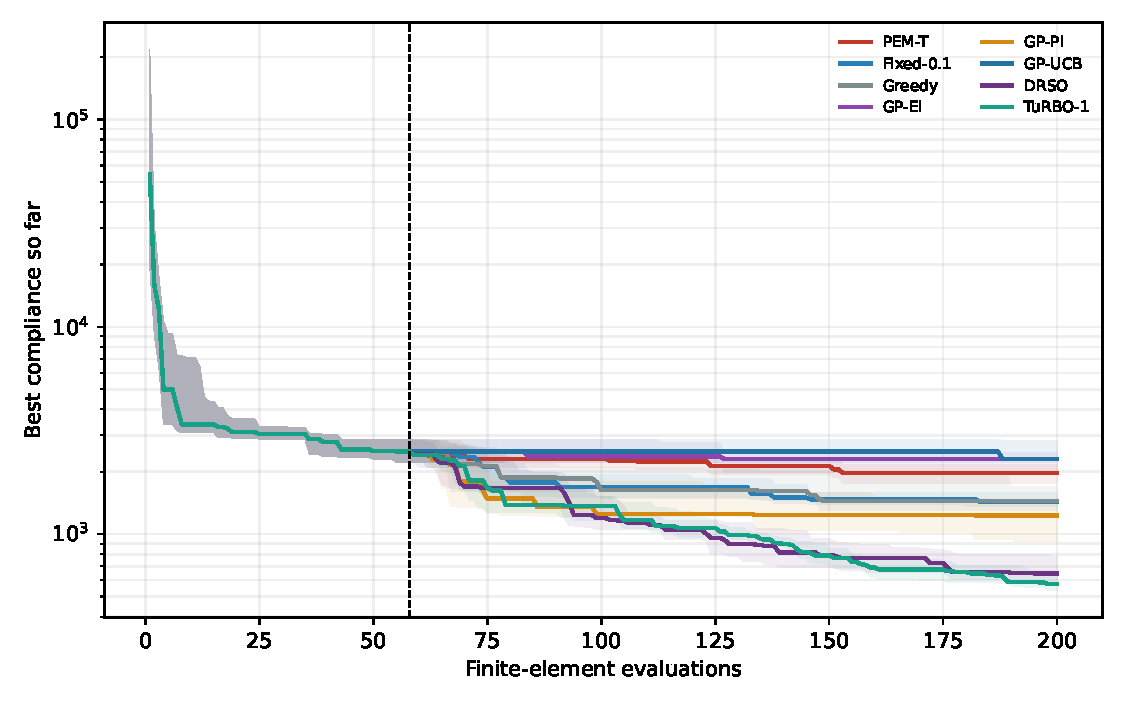
\includegraphics[width=0.92\textwidth]{figures/main_figure_4.pdf}
\caption{Median and interquartile best-so-far finite-element compliance under a shared 58-point initialization; the dashed line marks the end of initialization.}
\label{fig:main-4}
\end{figure}

Figure 4 separates the common initialization from method-specific search. All curves share the same values up to the dashed 58-evaluation boundary. TuRBO-1 and DRSO then improve rapidly and reach the lowest endpoint group. GP-PI also produces sustained improvement and finishes below the three internal methods, whereas GP-EI and GP-UCB show little median improvement after initialization. Greedy and fixed01 improve more gradually and remain below PEM-T near the endpoint. The shaded interquartile bands preserve between-repeat variability and show that the endpoint ordering is not produced by a single trajectory.

Representative endpoint density fields for all eight shared-initialization methods are shown on the common material-density scale in Figure 5.

\begin{figure}[H]
\centering
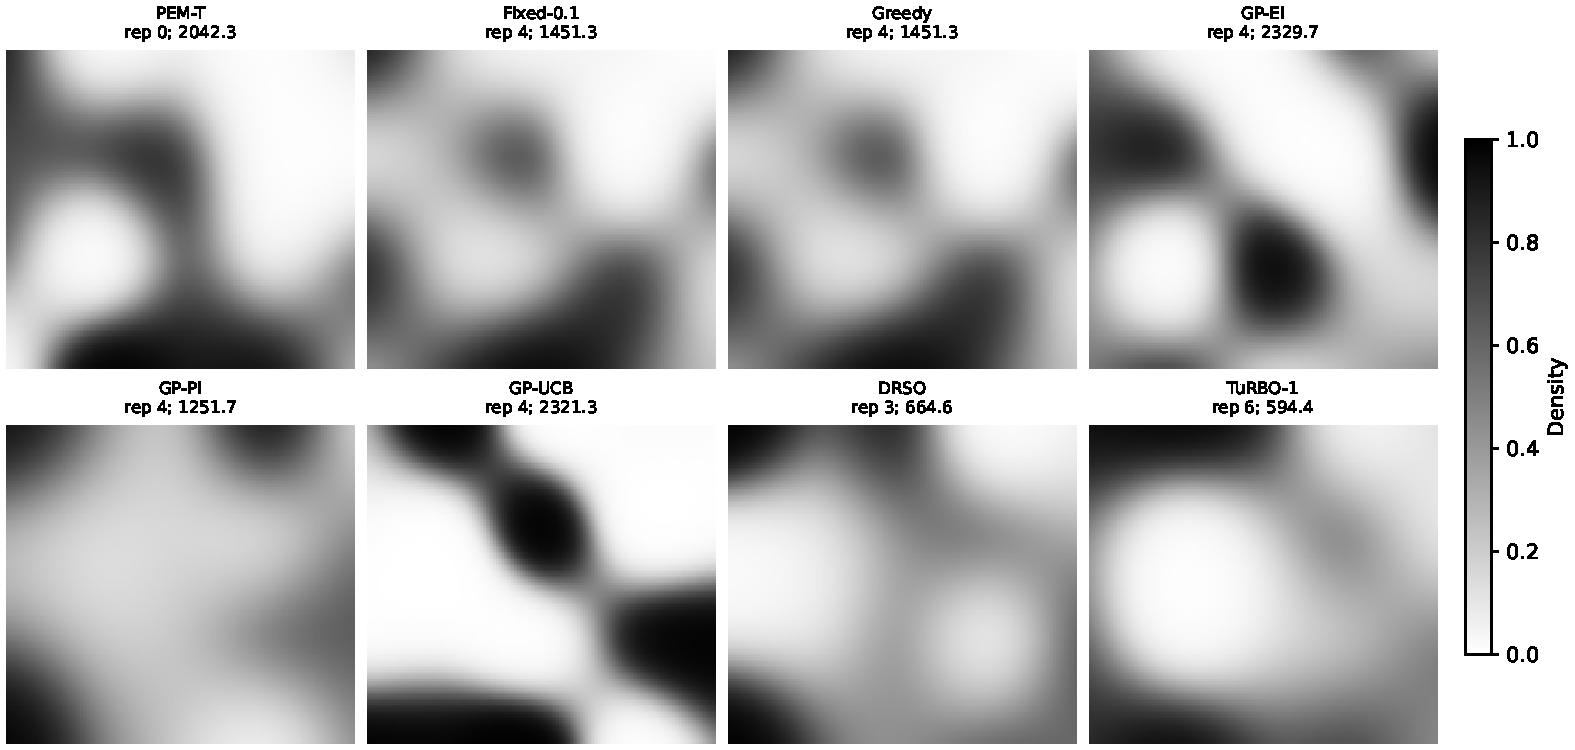
\includegraphics[width=0.98\textwidth]{figures/main_figure_5.pdf}
\caption{Representative median-run density fields for all eight methods under the shared-initialization comparison.}
\label{fig:main-5}
\end{figure}

Figure 5 shows the median-endpoint design from every method on the common density scale. Because every field satisfies the same mean-density constraint, the contrast concerns material placement rather than material quantity. TuRBO-1 and DRSO form concentrated high-density load paths and reach the lowest compliance group. GP-PI produces a stronger structural path than GP-EI or GP-UCB, whose diffuse fields remain close to their initial designs. The visual differences are consistent with the convergence pathways and endpoint ordering in Table 4.

\hypertarget{discussion-and-design-guidance}{%
\section{Discussion and Design Guidance}\label{discussion-and-design-guidance}}

The deterministic and empirical findings answer different questions. Ordering redundancy follows from the stated decision rule and holds whenever the correction is common across supported candidates. The observed performance loss is specific to the tested feedback controller, surrogate, candidates, and budgets. It does not imply that candidate-dependent uncertainty, conformal Bayesian optimization, or all adaptive exploration is ineffective.

The results support a staged design procedure for surrogate model management. First, identify the exact route from the monitoring statistic to the decision. If the signal adds a common constant before an argmin, it cannot alter ranking. Second, freeze common states and compare the true utility of the alternative choices. This exposes an unhelpful exploration response before histories diverge. Third, run closed-loop validation on instances not used to select controls or coefficients. Calibration statistics remain useful diagnostics, but they should not serve as substitutes for either decision utility or final objective value.

The prototype illustrates why this sequence matters. Its failure fraction is close to 0.1, which could be read as successful monitoring. The same controller increases exploration from about 0.1 to 0.34-0.40, selects candidates with lower immediate improvement, and ends with larger errors. Localized weighting further improves some quantile-loss diagnostics without producing better trajectories. The missing link is not error measurement; it is a rule connecting error information to valuable evaluations.

For engineering users, the practical implication is to evaluate the acquisition pathway before paying for large simulation batches. A useful monitor should make candidate-specific distinctions that align with objective improvement, or it should govern an evaluation gate, restart, or stopping decision whose value can be tested. Monitoring width or error merely to increase exploration can consume the same number of expensive evaluations in less productive regions.

The study has limitations. Residuals originate from changing surrogate models and scales; no exchangeability argument establishes pointwise coverage. Sparse declarations limit conditional reliability statements. The RBF surrogate truncates training data, and the candidate process is one implementation among many. The broad BBOB external-reference batches retain their native initialization, although the finite-element sensitivity analysis removes this difference. The beam study uses a smooth 19-dimensional design family, not unrestricted 5,000-variable topology optimization. Full sensitivity, 300-dimensional, application, resource, and recovery evidence is supplied separately so that these limits remain auditable without dominating the main paper.

\hypertarget{conclusion}{%
\section{Conclusion}\label{conclusion}}

A decision-consequence auditing framework has been developed for reliability assessment in surrogate-assisted optimization. It makes the path from surrogate-derived information to model-management action explicit and requires separate evidence for calibration, decision influence, common-state utility, and closed-loop optimization. The ranking-invariance criterion and prediction-before-label protocol allow structurally redundant mechanisms and information leakage to be identified before large experimental budgets are committed.

The temporal residual monitor illustrates the framework rather than defining its scope. Its aggregate failure rate is close to the nominal level, but its candidate-independent correction cannot create a distinct exploitation ranking, its feedback choices have lower immediate utility, and its held-out BBOB and finite-element trajectories do not pass the optimization-benefit gate. The shared-initialization controls sharpen this interpretation: GP-PI, author-code DRSO, and TuRBO-1 produce strong improvement, whereas GP-EI and fixed-multiplier GP-UCB do not improve the median initial incumbent. These outcomes show that the audit can distinguish actionable Bayesian, evolutionary-surrogate, and trust-region management from mechanisms whose plausible uncertainty signal does not translate into valuable evaluations.

The framework is intended as a predeployment screen for expensive engineering optimization. Applying its stages in order can prevent calibration statistics from being mistaken for optimization value, focus simulation resources on mechanisms with an identifiable decision path, and retain a reproducible record of why a surrogate-management component was promoted, revised, or stopped.

\acknowledgement{During the preparation of this manuscript, OpenAI Codex was used only for copyediting and language refinement to improve spelling, grammar, clarity, and flow. The research questions, experimental protocols, acceptance criteria, software, and scientific interpretations were produced by the authors. The authors reviewed and edited all affected text and take full responsibility for the content of the article.}
\funding{The authors received no specific funding for this study.}
\authorcontributions{The authors confirm contribution to the paper as follows: conceptualization, Ya-Yu Zhang and Shu-Chuan Chu; methodology, Ya-Yu Zhang, Shu-Chuan Chu, and Zhenyu Meng; software, Ya-Yu Zhang; validation, Ya-Yu Zhang, Zhenyu Meng, and Zhao Jia; formal analysis, Ya-Yu Zhang and Zhenyu Meng; investigation, Ya-Yu Zhang and Zhao Jia; data curation, Ya-Yu Zhang; visualization, Ya-Yu Zhang and Zhao Jia; writing---original draft preparation, Ya-Yu Zhang; writing---review and editing, Shu-Chuan Chu, Zhenyu Meng, Zhao Jia, and Ya-Yu Zhang; supervision, Shu-Chuan Chu; project administration, Shu-Chuan Chu. All authors reviewed the results and approved the final version of the manuscript.}
\availabilityofdataandmaterials{The data and code supporting the findings of this study are available from the corresponding author upon reasonable request during peer review and will be deposited in the public GitHub repository upon acceptance.}
\ethicsapproval{Not applicable. This study did not involve human participants or animals.}
\conflictsofinterest{The authors declare no conflicts of interest to report regarding the present study.}
\supplementary{The supplementary document contains full function-level results, LassoBench and 300-dimensional transfer evidence, model and budget sensitivity studies, exclusive resource measurements, recovery accounting, and reproducibility audits.}
\reftitle{References}
\begin{thebibliography}{999}
\bibitem{ref-1}
Y. Jin, ``Surrogate-assisted evolutionary computation: Recent advances and future challenges,'' Swarm Evol. Comput., vol.~1, no. 2, pp.~61-70, 2011. doi: 10.1016/j.swevo.2011.05.001.
\bibitem{ref-2}
J. Liang, Y. Lou, M. Yu, Y. Bi, and K. Yu, ``A survey of surrogate-assisted evolutionary algorithms for expensive optimization,'' J. Membr. Comput., vol.~7, pp.~108-127, 2025. doi: 10.1007/s41965-024-00165-w.
\bibitem{ref-3}
D. R. Jones, M. Schonlau, and W. J. Welch, ``Efficient global optimization of expensive black-box functions,'' J. Glob. Optim., vol.~13, pp.~455-492, 1998. doi: 10.1023/A:1008306431147.
\bibitem{ref-4}
Y. Jin, H. Wang, T. Chugh, D. Guo, and K. Miettinen, ``Data-driven evolutionary optimization: An overview and case studies,'' IEEE Trans. Evol. Comput., vol.~23, no. 3, pp.~442-458, 2019.
\bibitem{ref-5}
J.-Y. Li, Z.-H. Zhan, and J. Zhang, ``Evolutionary computation for expensive optimization: A survey,'' Int. J. Autom. Comput., vol.~18, pp.~1-21, 2021.
\bibitem{ref-6}
H. Zou, S. Zeng, C. Li, R. Jiao, and F. Zhao, ``Uncertainty estimation by boosting with Gaussian process for expensive optimization problems,'' Appl. Soft Comput., vol.~180, Art. no. 113320, 2025. doi: 10.1016/j.asoc.2025.113320.
\bibitem{ref-7}
Y. Li, Y. Zhuang, Y. Li, J. Fan, L. Wang, Y. Qi, J. Xiong, and X. Ma, ``A surrogate-assisted evolutionary algorithm with Gaussian process regression and diversity search for large-scale expensive optimization,'' Appl. Soft Comput., vol.~182, Art. no. 113440, 2025. doi: 10.1016/j.asoc.2025.113440.
\bibitem{ref-8}
X. Yang et al., ``A surrogate-assisted differential evolution algorithm with a dual-space-driven selection strategy for expensive optimization problems,'' Complex Intell. Syst., vol.~11, Art. no. 230, 2025. doi: 10.1007/s40747-025-01812-0.
\bibitem{ref-9}
R. Zhou, C. Ren, Z. Meng, and H. Zhu, ``Surrogate-assisted differential evolution with search space tightening for high-dimensional expensive optimization problems,'' IEEE Trans. Syst. Man Cybern. Syst., vol.~55, no. 10, pp.~7356-7368, 2025. doi: 10.1109/TSMC.2025.3582897.
\bibitem{ref-10}
L. Yu, Y. Guo, L. Feng, Z. Zhu, Z. Wei, and Y. Hou, ``A multi-source surrogate-assisted evolutionary algorithm for expensive optimization: An optinformatics perspective,'' Swarm Evol. Comput., vol.~107, Art. no. 102491, 2026. doi: 10.1016/j.swevo.2026.102491.
\bibitem{ref-11}
Q. Liu, X. Wu, Q. Lin, J. Ji, and K.-C. Wong, ``A novel surrogate-assisted evolutionary algorithm with an uncertainty grouping based infill criterion,'' Swarm Evol. Comput., vol.~60, Art. no. 100787, 2021.
\bibitem{ref-12}
S. Deshpande, C. Marx, and V. Kuleshov, ``Online calibrated and conformal prediction improves Bayesian optimization,'' in Proc. AISTATS, PMLR, vol.~238, pp.~1450-1458, 2024.
\bibitem{ref-13}
D. Kim, M. Zecchin, S. Park, J. Kang, and O. Simeone, ``Robust Bayesian optimization via localized online conformal prediction,'' arXiv:2411.17387v2, 2025.
\bibitem{ref-14}
Y. Jin and Z. Ren, ``Confidence on the focal: Conformal prediction with selection-conditional coverage,'' arXiv:2403.03868v3, 2024.
\bibitem{ref-15}
E. Nardone, C. De Stefano, A. Scotto di Freca, F. Fontanella, and T. D'Alessandro, ``Toward reliable uncertainty quantification in surrogate-assisted evolutionary algorithms via temporal conformal prediction,'' in Applications of Evolutionary Computation, LNCS 16524, pp.~384-401, 2026. doi: 10.1007/978-3-032-23604-3\_24.
\bibitem{ref-16}
Y. S. Ong, P. B. Nair, and A. J. Keane, ``Evolutionary optimization of computationally expensive problems via surrogate modeling,'' AIAA J., vol.~41, no. 4, pp.~687-696, 2003.
\bibitem{ref-17}
H. Wang, Y. Jin, and J. Doherty, ``Committee-based active learning for surrogate-assisted particle swarm optimization of expensive problems,'' IEEE Trans. Cybern., vol.~47, no. 9, pp.~2664-2677, 2017.
\bibitem{ref-18}
M. Yu, X. Li, and J. Liang, ``A dynamic surrogate-assisted evolutionary algorithm framework for expensive structural optimization,'' Struct. Multidiscip. Optim., vol.~61, no. 2, pp.~711-729, 2020.
\bibitem{ref-19}
C. Sun, Y. Jin, R. Cheng, J. Ding, and J. Zeng, ``Surrogate-assisted cooperative swarm optimization of high-dimensional expensive problems,'' IEEE Trans. Evol. Comput., vol.~21, no. 4, pp.~644-660, 2017.
\bibitem{ref-20}
Y. Hanawa, T. Harada, and Y. Miura, ``Impact of surrogate model accuracy on performance and model management strategy in surrogate-assisted evolutionary algorithms,'' Array, vol.~27, Art. no. 100461, 2025. doi: 10.1016/j.array.2025.100461.
\bibitem{ref-21}
M. Gobert, G. Briffoteaux, J. Gmys, N. Melab, and D. Tuyttens, ``Observations in applying Bayesian versus evolutionary approaches and their hybrids in parallel time-constrained optimization,'' Eng. Appl. Artif. Intell., vol.~137, Art. no. 109075, 2024. doi: 10.1016/j.engappai.2024.109075.
\bibitem{ref-22}
H. Hao, X. Zhang, and A. Zhou, ``Un-evaluated solutions may be valuable in expensive optimization,'' Swarm Evol. Comput., vol.~94, Art. no. 101905, 2025. doi: 10.1016/j.swevo.2025.101905.
\bibitem{ref-23}
F. Felten et al., ``EngiBench: A framework for data-driven engineering design research,'' in Adv. Neural Inf. Process. Syst., 2025. {[}Online{]}. Available: https://openreview.net/forum?id=YowD33Q89V.
\bibitem{ref-24}
K. Sehic, A. Gramfort, J. Salmon, and L. Nardi, ``LassoBench: A high-dimensional hyperparameter optimization benchmark suite for Lasso,'' in Proc. 1st Int. Conf. Automated Machine Learning, PMLR, vol.~188, pp.~2/1-2/24, 2022.
\bibitem{ref-25}
D. Eriksson, M. Pearce, J. Gardner, R. D. Turner, and M. Poloczek, ``Scalable global optimization via local Bayesian optimization,'' in Adv. Neural Inf. Process. Syst., vol.~32, 2019.
\bibitem{ref-26}
N. Hansen et al., ``COCO: A platform for comparing continuous optimizers in a black-box setting,'' Optim. Methods Softw., vol.~36, no. 1, pp.~114-144, 2021. doi: 10.1080/10556788.2018.1502028.
\bibitem{ref-27}
X. Liu, Y. Bao, and F. Leng, ``Neural architecture search via hierarchical evaluation of surrogate models,'' Comput. Mater. Contin., vol.~84, no. 2, pp.~3503-3517, 2025. doi: 10.32604/cmc.2025.064544.
\bibitem{ref-28}
S. Ibrayev, B. Omarov, A. Ibrayeva, and Z. Momynkulov, ``DeepSurNet-NSGA II: Deep surrogate model-assisted multi-objective evolutionary algorithm for enhancing leg linkage in walking robots,'' Comput. Mater. Contin., vol.~81, no. 1, pp.~229-249, 2024. doi: 10.32604/cmc.2024.053075.
\bibitem{ref-29}
Z. Wang, L. Duan, L. Kuang, H. Zhou, and J. Duan, ``Physics-informed Gaussian process regression with Bayesian optimization for laser welding quality control in coaxial laser diodes,'' Comput. Mater. Contin., vol.~84, no. 2, pp.~2587-2604, 2025. doi: 10.32604/cmc.2025.065648.
\bibitem{ref-30}
H. Hao, X. Q. Zhang, and A. M. Zhou, ``Enhancing SAEAs with unevaluated solutions: A case study of relation model for expensive optimization,'' Sci. China Inf. Sci., vol.~67, no. 2, Art. no. 120103, 2024. doi: 10.1007/s11432-023-3909-x.
\bibitem{ref-31}
J.-S. Pan, J. Chen, J. Li, and Z. Meng, ``Differential evolution with exponential crossover: A survey,'' Comput. Sci. Rev., vol.~62, Art. no. 100990, 2026. doi: 10.1016/j.cosrev.2026.100990.
\bibitem{ref-32}
J.-S. Pan, Y. Peng, J. Li, J. Zhao, L. Kong, and S.-C. Chu, ``Multilayer perceptron grouping and sparse Gaussian process-based surrogate-assisted evolutionary algorithm for expensive multiobjective optimization,'' IEEE Trans. Cybern., vol.~56, no. 4, pp.~2148-2161, 2026. doi: 10.1109/TCYB.2025.3634364.
\bibitem{ref-33}
R.-Y. Wang, J.-S. Pan, S.-C. Chu, V. Snášel, J. Zhao, and H.-M. Yang, ``A bimodal surrogate-assisted PSO algorithm with wide coverage and dynamic space refinement for expensive multi-UAV path planning,'' Expert Syst. Appl., vol.~331, Art. no. 133075, 2026. doi: 10.1016/j.eswa.2026.133075.
\end{thebibliography}
\end{document}
